\documentclass[aspectratio=169]{beamer}

\usetheme{Madrid}
\usecolortheme{default}

\usepackage[T1]{fontenc}
\usepackage[utf8]{inputenc}
\usepackage{amsmath}
\usepackage{amssymb}
\usepackage{bm}
\usepackage{booktabs}
\usepackage{graphicx}
\usepackage{tikz}
\usepackage{array}

\graphicspath{{../figures/}{../figures/presentation/}}

\definecolor{ThesisBlue}{RGB}{47,111,159}
\definecolor{ThesisGreen}{RGB}{75,143,90}
\definecolor{ThesisRed}{RGB}{200,74,58}
\definecolor{ThesisGold}{RGB}{217,164,65}
\definecolor{ThesisGray}{RGB}{75,85,99}

\setbeamercolor{structure}{fg=ThesisBlue}
\setbeamercolor{frametitle}{bg=ThesisBlue,fg=white}
\setbeamercolor{title}{fg=ThesisBlue}
\setbeamercolor{block title}{bg=ThesisBlue!12,fg=ThesisBlue}
\setbeamercolor{block body}{bg=ThesisBlue!4,fg=black}
\setbeamertemplate{navigation symbols}{}
\setbeamertemplate{itemize item}{\color{ThesisBlue}$\blacktriangleright$}
\setbeamertemplate{itemize subitem}{\color{ThesisBlue}$\circ$}

\newcommand{\smallcite}[1]{\vspace{0.2em}{\scriptsize\color{ThesisGray}#1}}
\newcommand{\takeaway}[1]{%
  \begin{block}{Takeaway}
    #1
  \end{block}
}

\title[Training set optimization]{Training set optimization for genomic prediction across island populations}
\author{Simen Nesland}
\date{April 2026}

\begin{document}

\begin{frame}[plain]
  \centering
  \vspace{1.4cm}
  {\LARGE\bfseries\color{ThesisBlue} Training set optimization for genomic prediction across island populations\par}
  \vspace{1.1cm}
  {\large Simen Nesland\par}
  \vspace{0.35cm}
  {\normalsize April 2026\par}
\end{frame}

\begin{frame}{Content}
  \begin{enumerate}
    \item \textbf{SNPs and phenotypes}
    \item \textbf{Genomic prediction}
    \item \textbf{When genomic prediction gets hard}
    \item \textbf{Training set optimization}
    \item \textbf{Reflections}
  \end{enumerate}
\end{frame}

\begin{frame}{SNPs and phenotypes}
  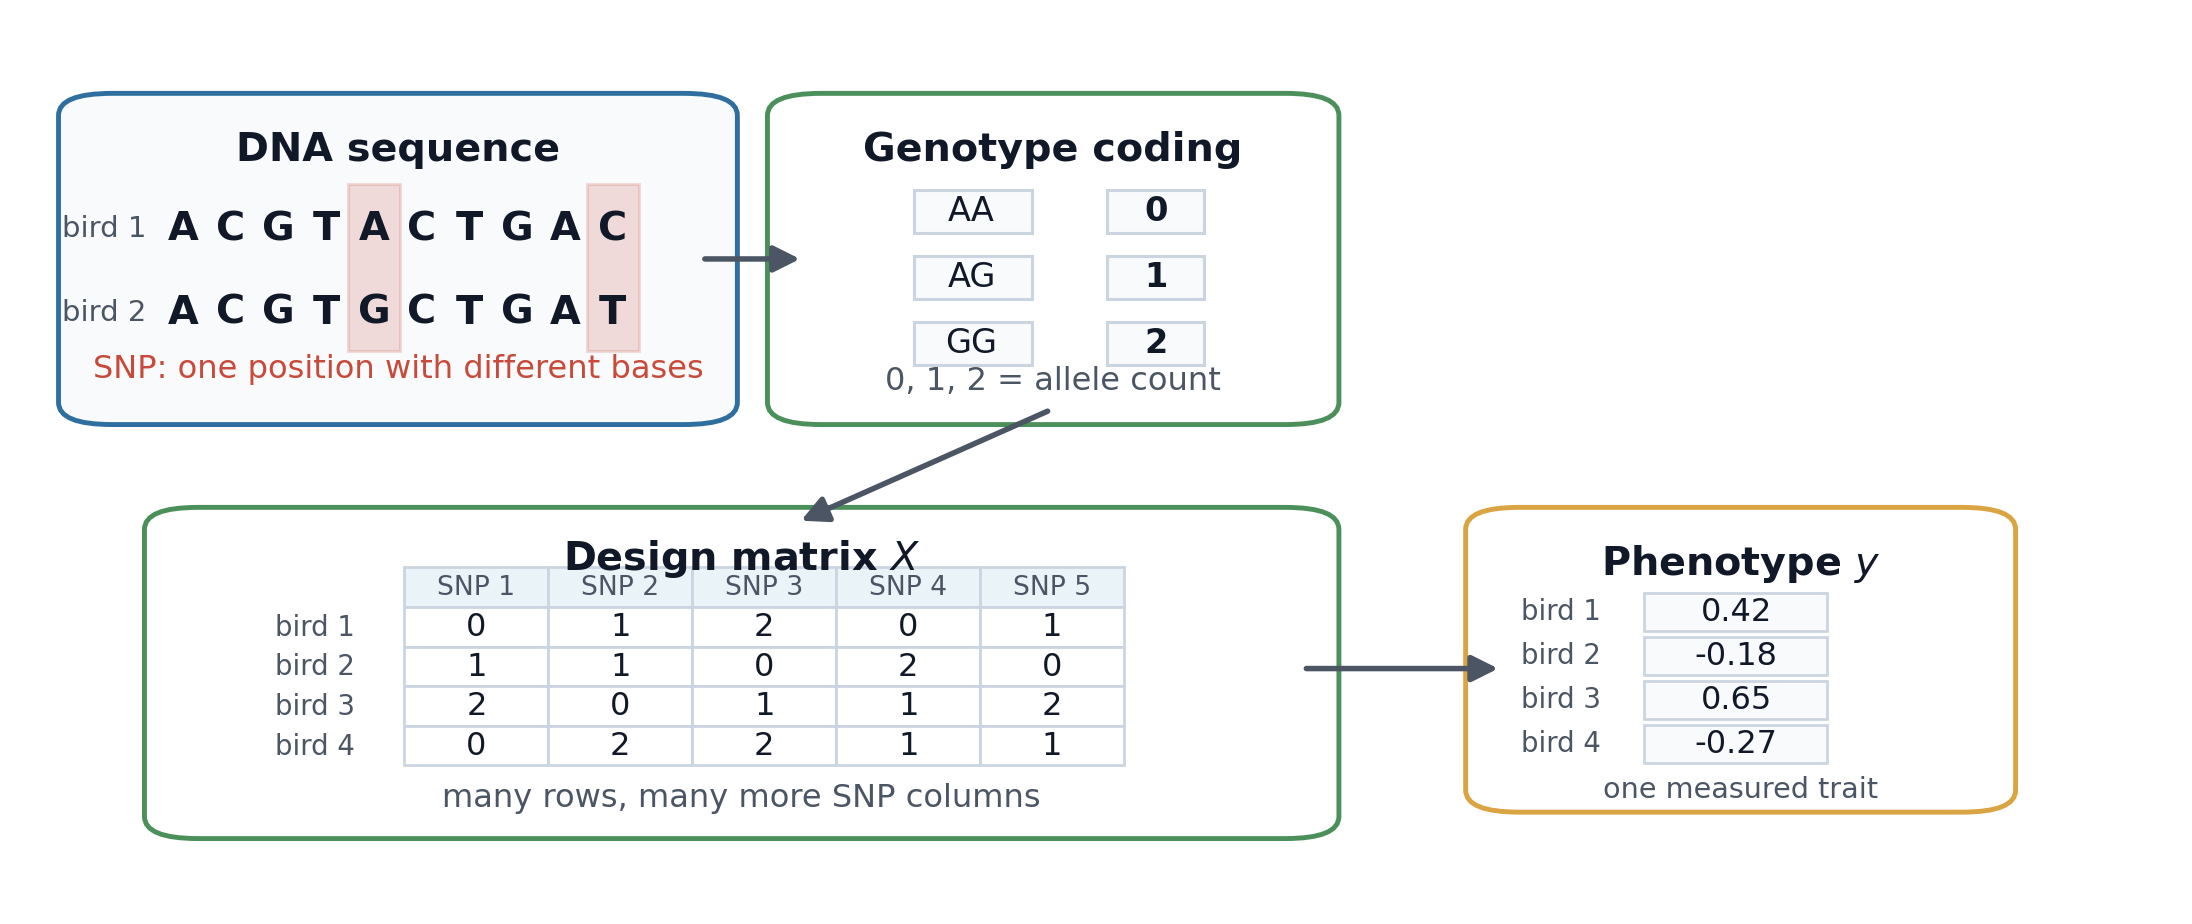
\includegraphics[width=\linewidth,height=0.78\textheight,keepaspectratio]{snp_to_prediction_schematic.png}
\end{frame}

\begin{frame}{Genomic prediction}
  \begin{columns}[T,onlytextwidth]
    \begin{column}{0.46\textwidth}
      \[
      \begin{array}{c|ccccc}
       & \text{SNP}_1 & \text{SNP}_2 & \text{SNP}_3 & \cdots & \text{SNP}_p\\
      \hline
      \text{bird }1 & 0 & 1 & 2 & \cdots & 0\\
      \text{bird }2 & 1 & 1 & 0 & \cdots & 2\\
      \text{bird }3 & 2 & 0 & 1 & \cdots & 1\\
      \vdots & \vdots & \vdots & \vdots & & \vdots
      \end{array}
      \]
      \[
        X_{ij}\in\{0,1,2\}, \qquad y_i=\text{measured trait}.
      \]
      \small The prediction problem is ordinary regression in an unusual regime: very many marker columns, fewer phenotyped individuals, and correlated columns.
    \end{column}
    \begin{column}{0.50\textwidth}
      \begin{block}{Marker-based regression}
      \[
        \bm{y}=\mu\mathbf{1}+X\bm{\beta}+\bm{\varepsilon}.
      \]
      Each \(\beta_j\) is the fitted effect of one SNP column.
      \end{block}
      \begin{block}{Mixed-model view}
      \[
        y_i=\mu+g_i+\varepsilon_i,\qquad
        g_i=x_i^\top\bm{\beta}.
      \]
      The genetic part \(g_i\) is latent, but the SNPs give us a high-dimensional proxy for it.
      \end{block}
      {\small
      \[
        \hat{\bm{\beta}}=
        \arg\min_{\bm{\beta}}
        \{\|\bm{y}-X\bm{\beta}\|_2^2+\lambda\|\bm{\beta}\|_2^2\}.
      \]
      }
    \end{column}
  \end{columns}
\end{frame}

\begin{frame}{Prediction engines: ridge and BPCRR}
  \begin{columns}[T,onlytextwidth]
    \begin{column}{0.48\textwidth}
      \begin{block}{Ridge}
      Fit all marker effects with a common shrinkage penalty.
      \[
        \hat y_*=\hat\mu+x_*^\top\hat{\bm{\beta}}.
      \]
      It is simple, stable, and a strong baseline in high dimensions.
      \end{block}
    \end{column}
    \begin{column}{0.48\textwidth}
      \begin{block}{BPCRR}
      Compress SNPs to principal components:
      \[
        Z=XU_q, \qquad q\ll p.
      \]
      Then fit a Bayesian ridge model in PC space:
      \[
        \bm{y}=\mu\mathbf{1}+Z\bm{\gamma}+\bm{\varepsilon}.
      \]
      \end{block}
    \end{column}
  \end{columns}

  \vspace{0.5em}
  \takeaway{Both are regularized linear prediction models; they differ mainly in whether shrinkage happens in marker space or PC space.}
\end{frame}

\begin{frame}{When genomic prediction gets hard}
  \begin{columns}[T,onlytextwidth]
    \begin{column}{0.50\textwidth}
      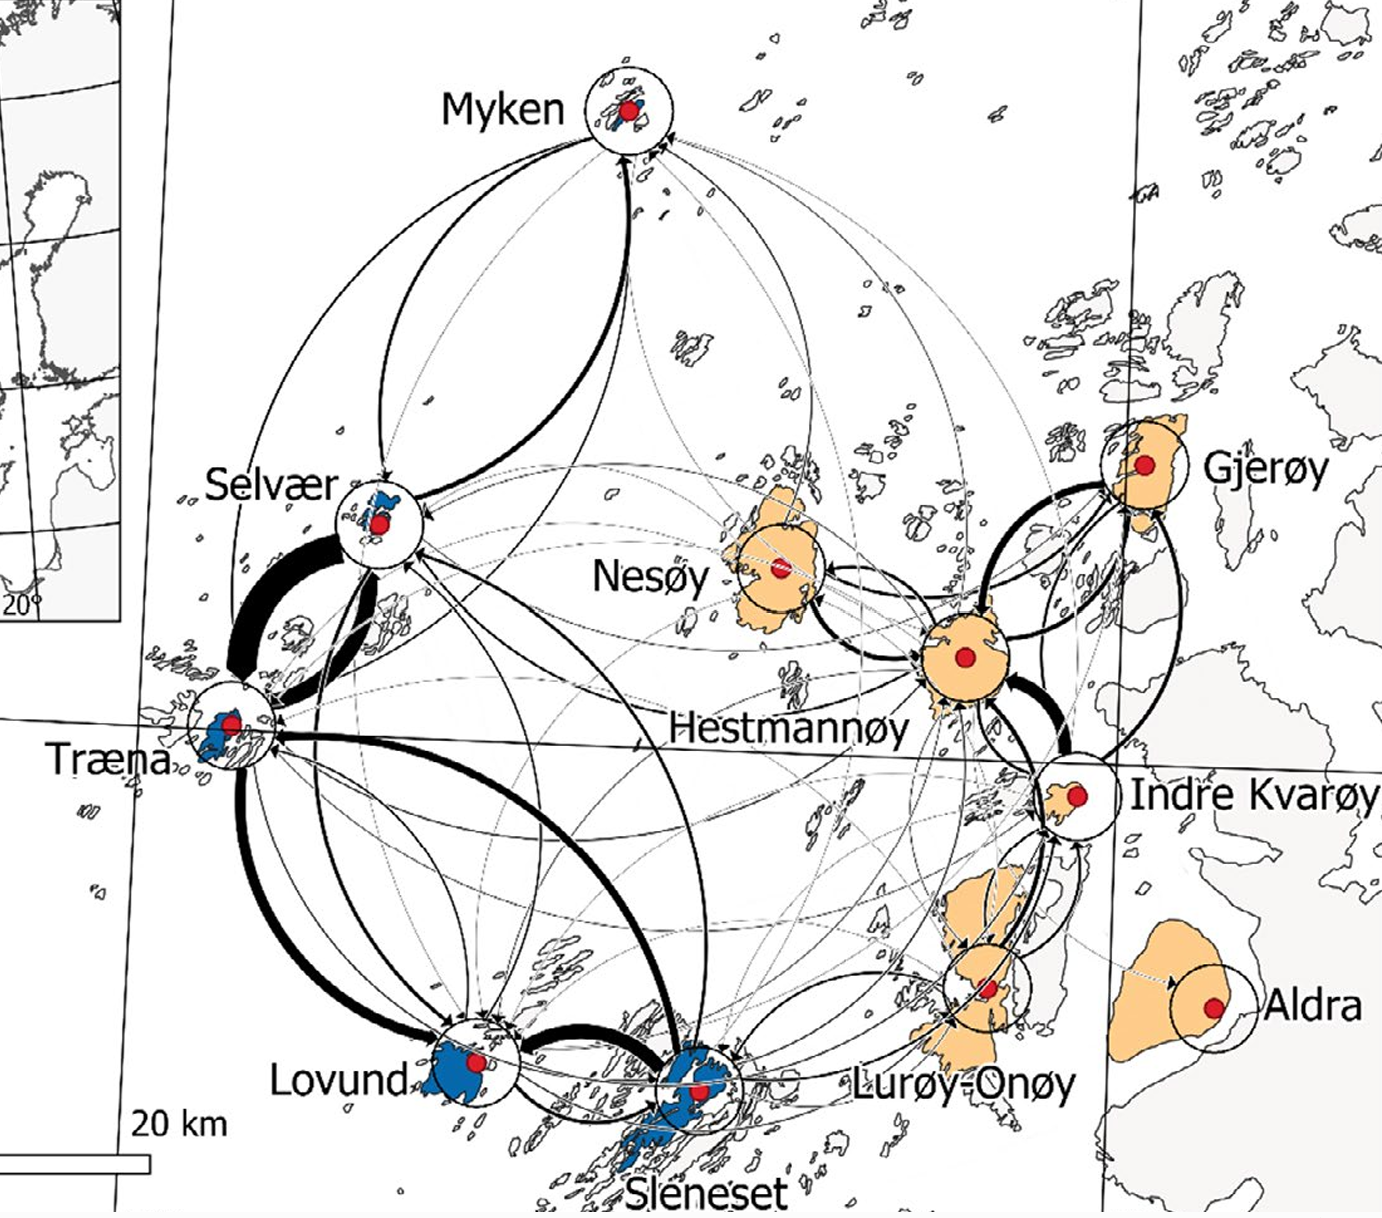
\includegraphics[width=\linewidth,height=0.66\textheight,keepaspectratio]{Islands.png}
    \end{column}
    \begin{column}{0.47\textwidth}
      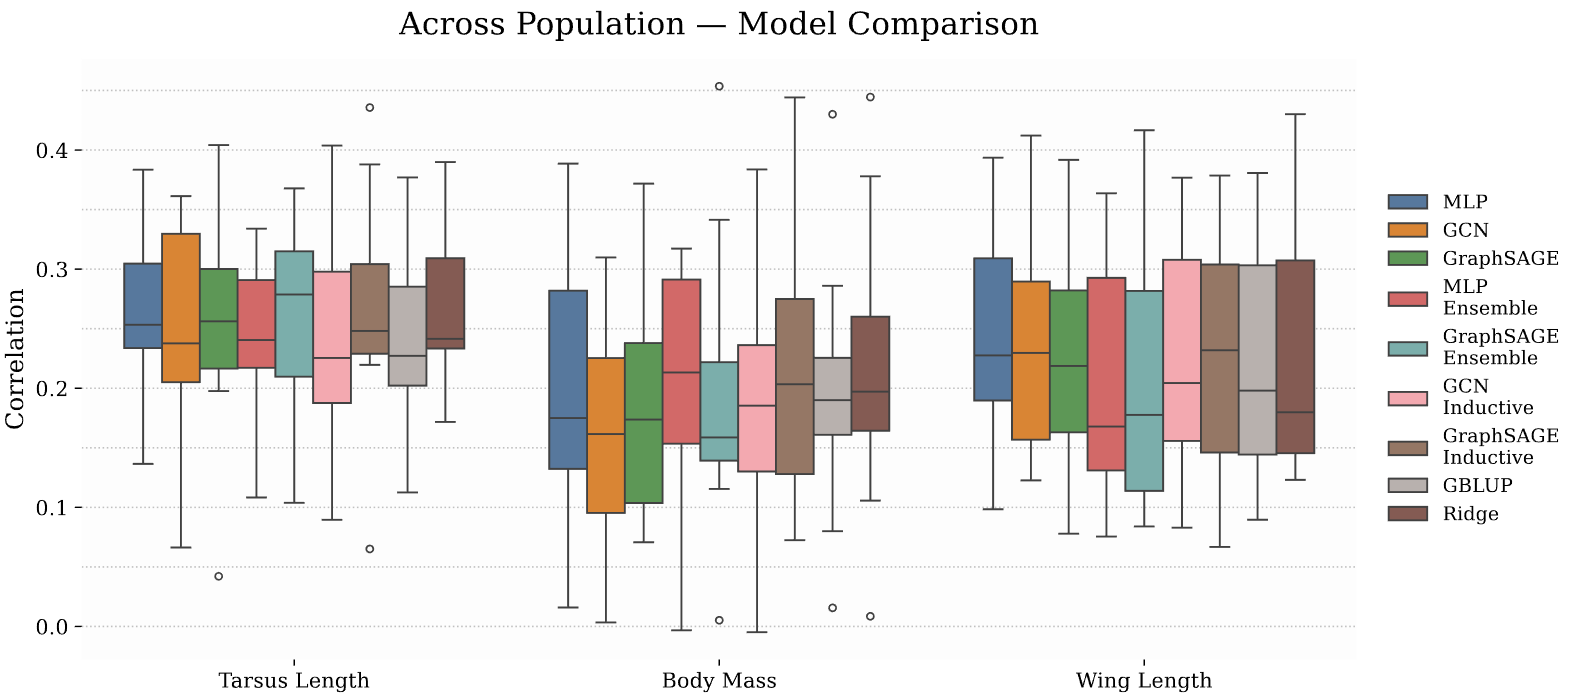
\includegraphics[width=\linewidth]{loio_single_panel.png}
      \vspace{0.2em}
      \small
      \begin{itemize}
        \item Within-population validation is close to ordinary supervised learning.
        \item Across-population prediction is a distribution-shift problem.
        \item In my data, the island structure gives a natural leave-one-island-out test.
      \end{itemize}
    \end{column}
  \end{columns}
\end{frame}

\begin{frame}{Training set optimization}
  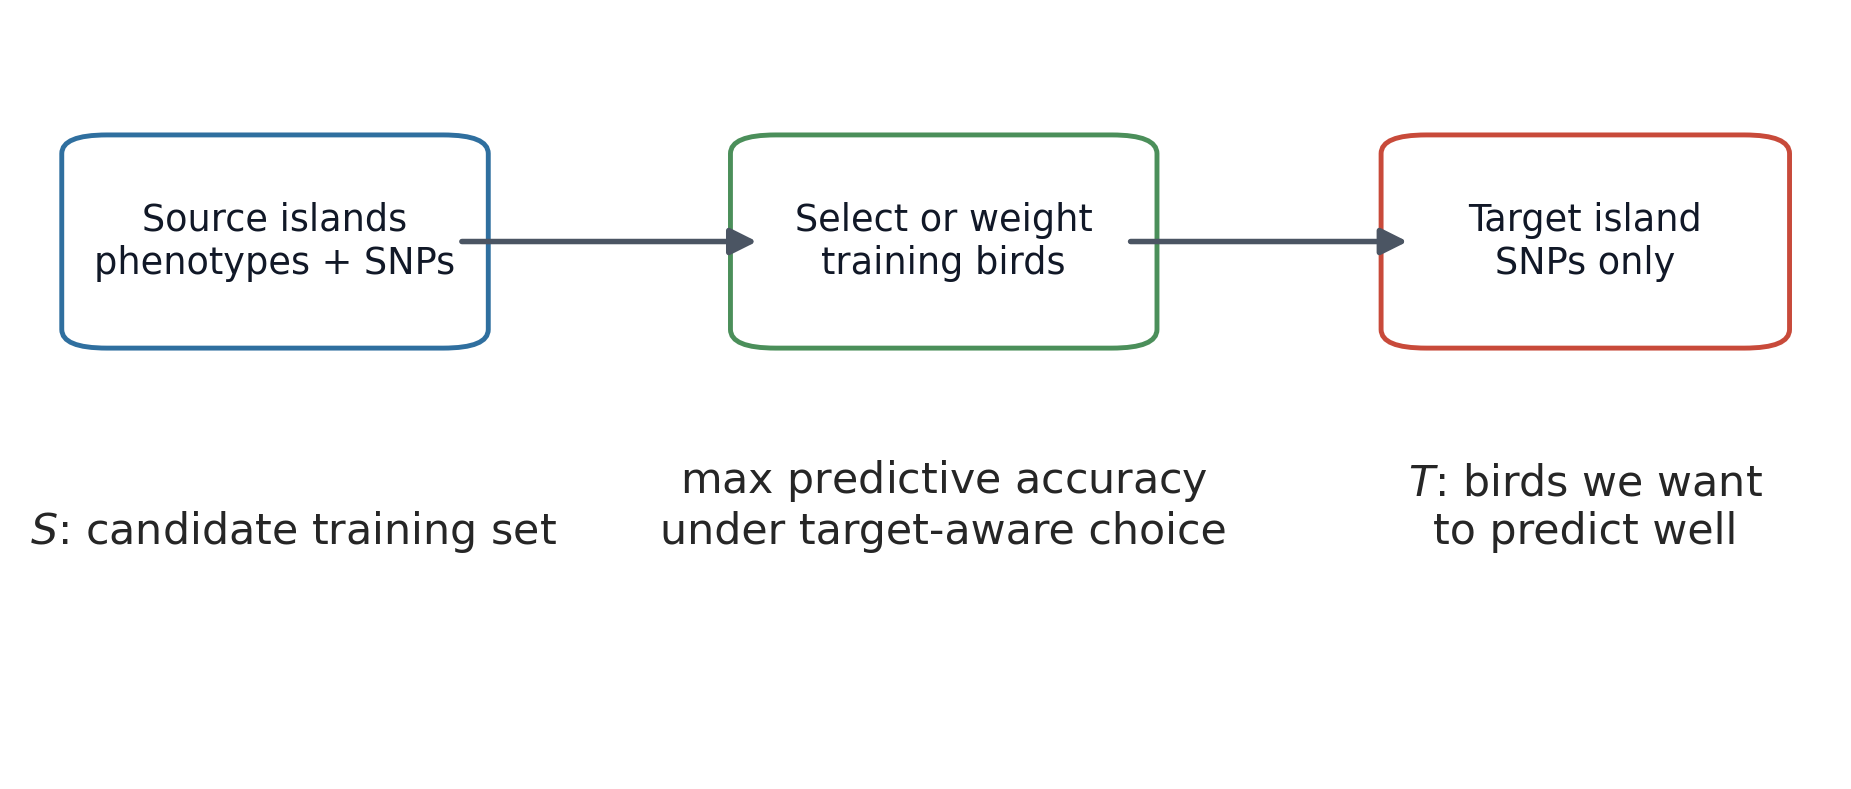
\includegraphics[width=\linewidth,height=0.42\textheight,keepaspectratio]{training_set_optimization_flow.png}

  \vspace{0.4em}
  \begin{columns}[T,onlytextwidth]
    \begin{column}{0.32\textwidth}
      \begin{block}{Goal}
      Predict a target island \(T\) using source islands with phenotypes and SNPs.
      \end{block}
    \end{column}
    \begin{column}{0.32\textwidth}
      \begin{block}{Choice}
      Choose a subset \(S_k\) or weights \(w_i\) before fitting ridge/BPCRR.
      \end{block}
    \end{column}
    \begin{column}{0.32\textwidth}
      \begin{block}{Constraint}
      In deployment, \(X_T\) is available but the target phenotypes \(y_T\) are not.
      \end{block}
    \end{column}
  \end{columns}

  \vspace{0.2em}
  \[
    \text{target-aware training:}\qquad
    \max_{S_k\ \text{or}\ w}\ \operatorname{cor}\{y_T,\hat y_T\}.
  \]
\end{frame}

\begin{frame}{Three routes I tried}
  \renewcommand{\arraystretch}{1.25}
  \begin{tabular}{>{\raggedright\arraybackslash}p{0.23\textwidth}
                  >{\raggedright\arraybackslash}p{0.39\textwidth}
                  >{\raggedright\arraybackslash}p{0.27\textwidth}}
    \toprule
    Method & Idea & What information it uses \\
    \midrule
    Data Shapley & Estimate each source island's marginal contribution to target prediction. & Genotypes, source phenotypes, and calibration target phenotypes. \\
    Top-\(k\) selection & Rank source candidates by genetic closeness or expected prediction uncertainty. & Genotypes and target SNPs. \\
    Importance weighting & Reweight source data to make the training distribution look more target-like. & Genotypes and target SNPs. \\
    \bottomrule
  \end{tabular}

  \vspace{0.8em}
  All results are evaluated with leave-one-island-out prediction and Pearson correlation on the held-out island.
\end{frame}

\begin{frame}{Data Shapley}
  \begin{columns}[T,onlytextwidth]
    \begin{column}{0.48\textwidth}
      \[
      \phi_i
      =
      \mathbb{E}_{S\subseteq D\setminus\{i\}}
      \left[
        V(S\cup\{i\})-V(S)
      \right].
      \]
      \begin{itemize}
        \item \(V(S)\): prediction performance when training on subset \(S\).
        \item I used island-wise TMC Shapley to make it computationally feasible.
        \item Useful diagnostically, but calibration target phenotypes make it partly oracle-like.
      \end{itemize}
      \smallcite{Data Shapley: Ghorbani and Zou (2019).}
    \end{column}
    \begin{column}{0.50\textwidth}
      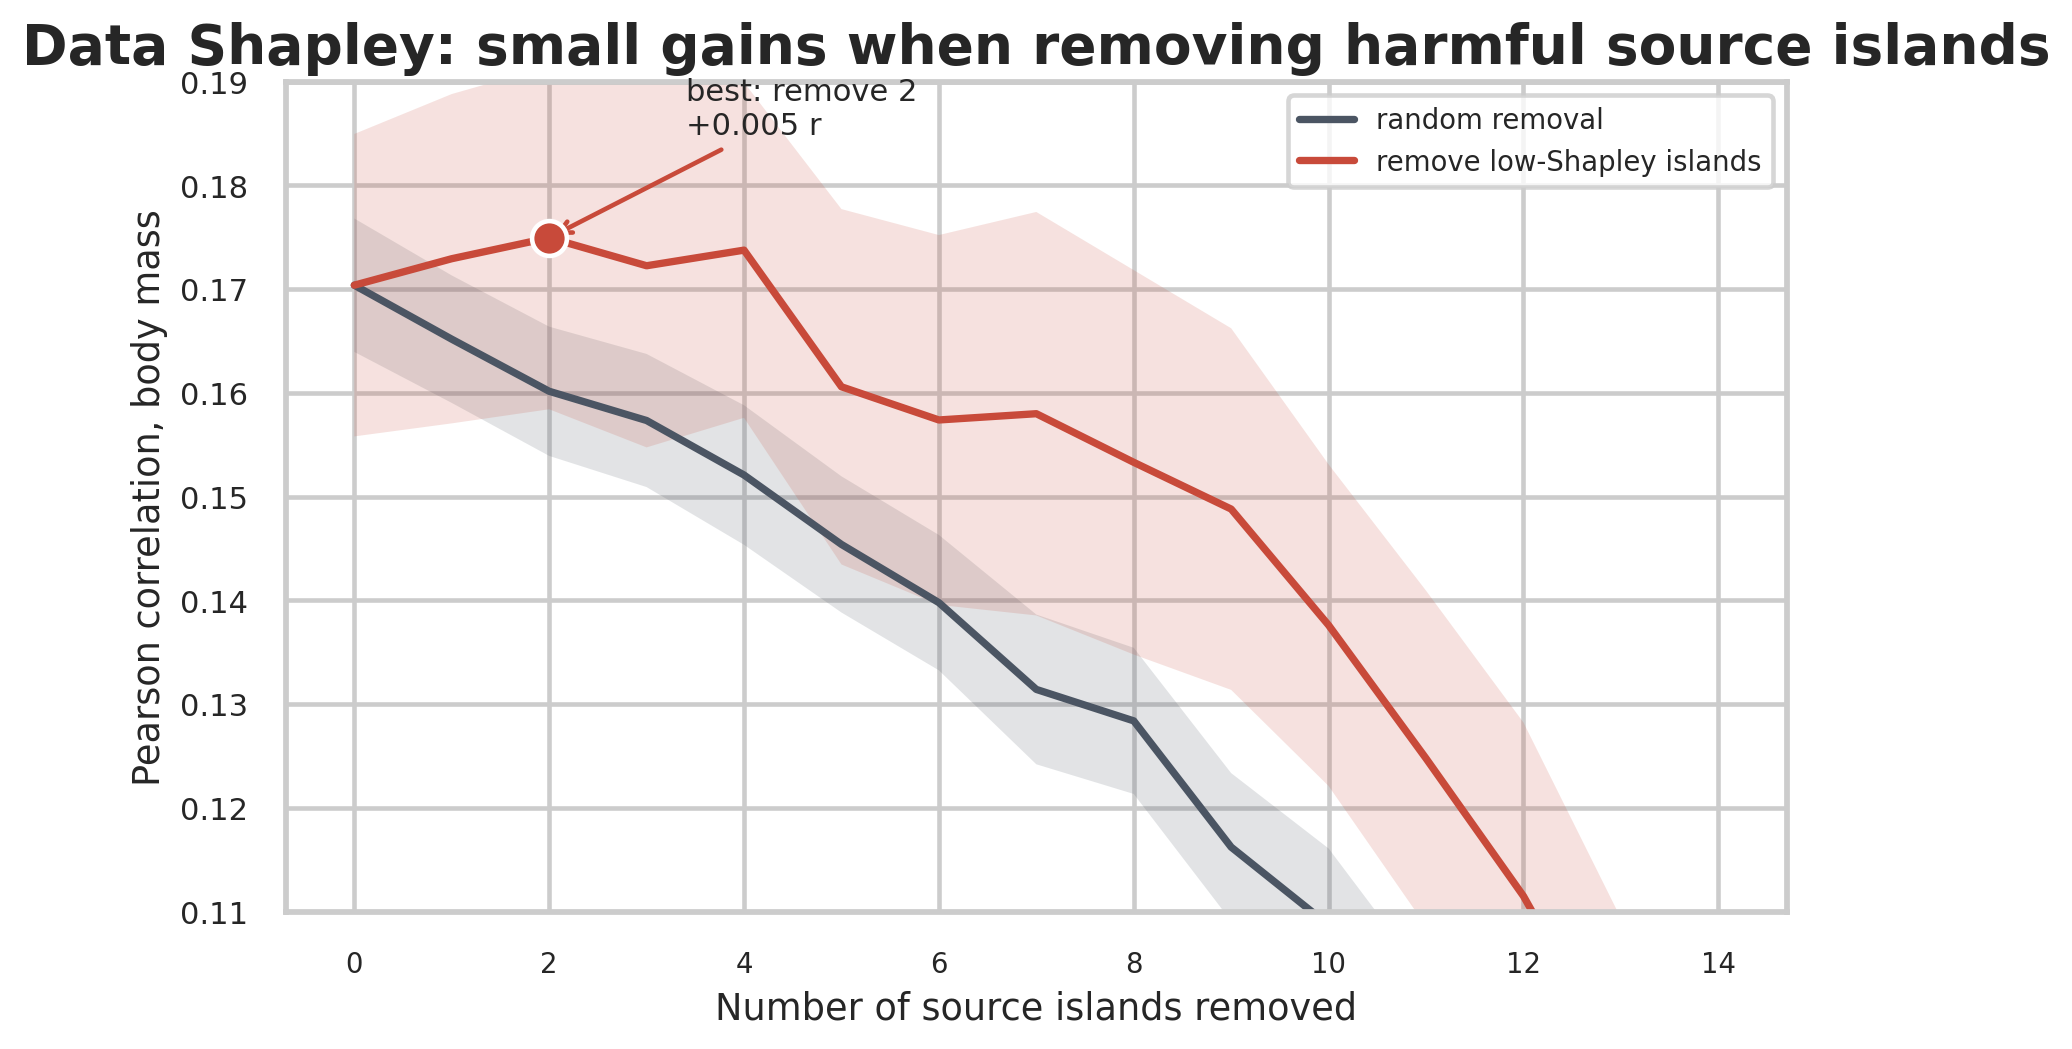
\includegraphics[width=\linewidth]{shapley_remove_curve_bodymass.png}
    \end{column}
  \end{columns}
\end{frame}

\begin{frame}{Top-\(k\) selection}
  \small
  \begin{columns}[T,onlytextwidth]
    \begin{column}{0.48\textwidth}
      Rank source candidate \(c\) by average genetic similarity to the target:
      \[
        s(c)=\frac{1}{|T|}\sum_{t\in T}G_{tc}
      \]
    \end{column}
    \begin{column}{0.48\textwidth}
      or in PC space:
      \[
        d(c)=\|z_c-\bar z_T\|_2.
      \]
    \end{column}
  \end{columns}

  \vspace{0.05em}
  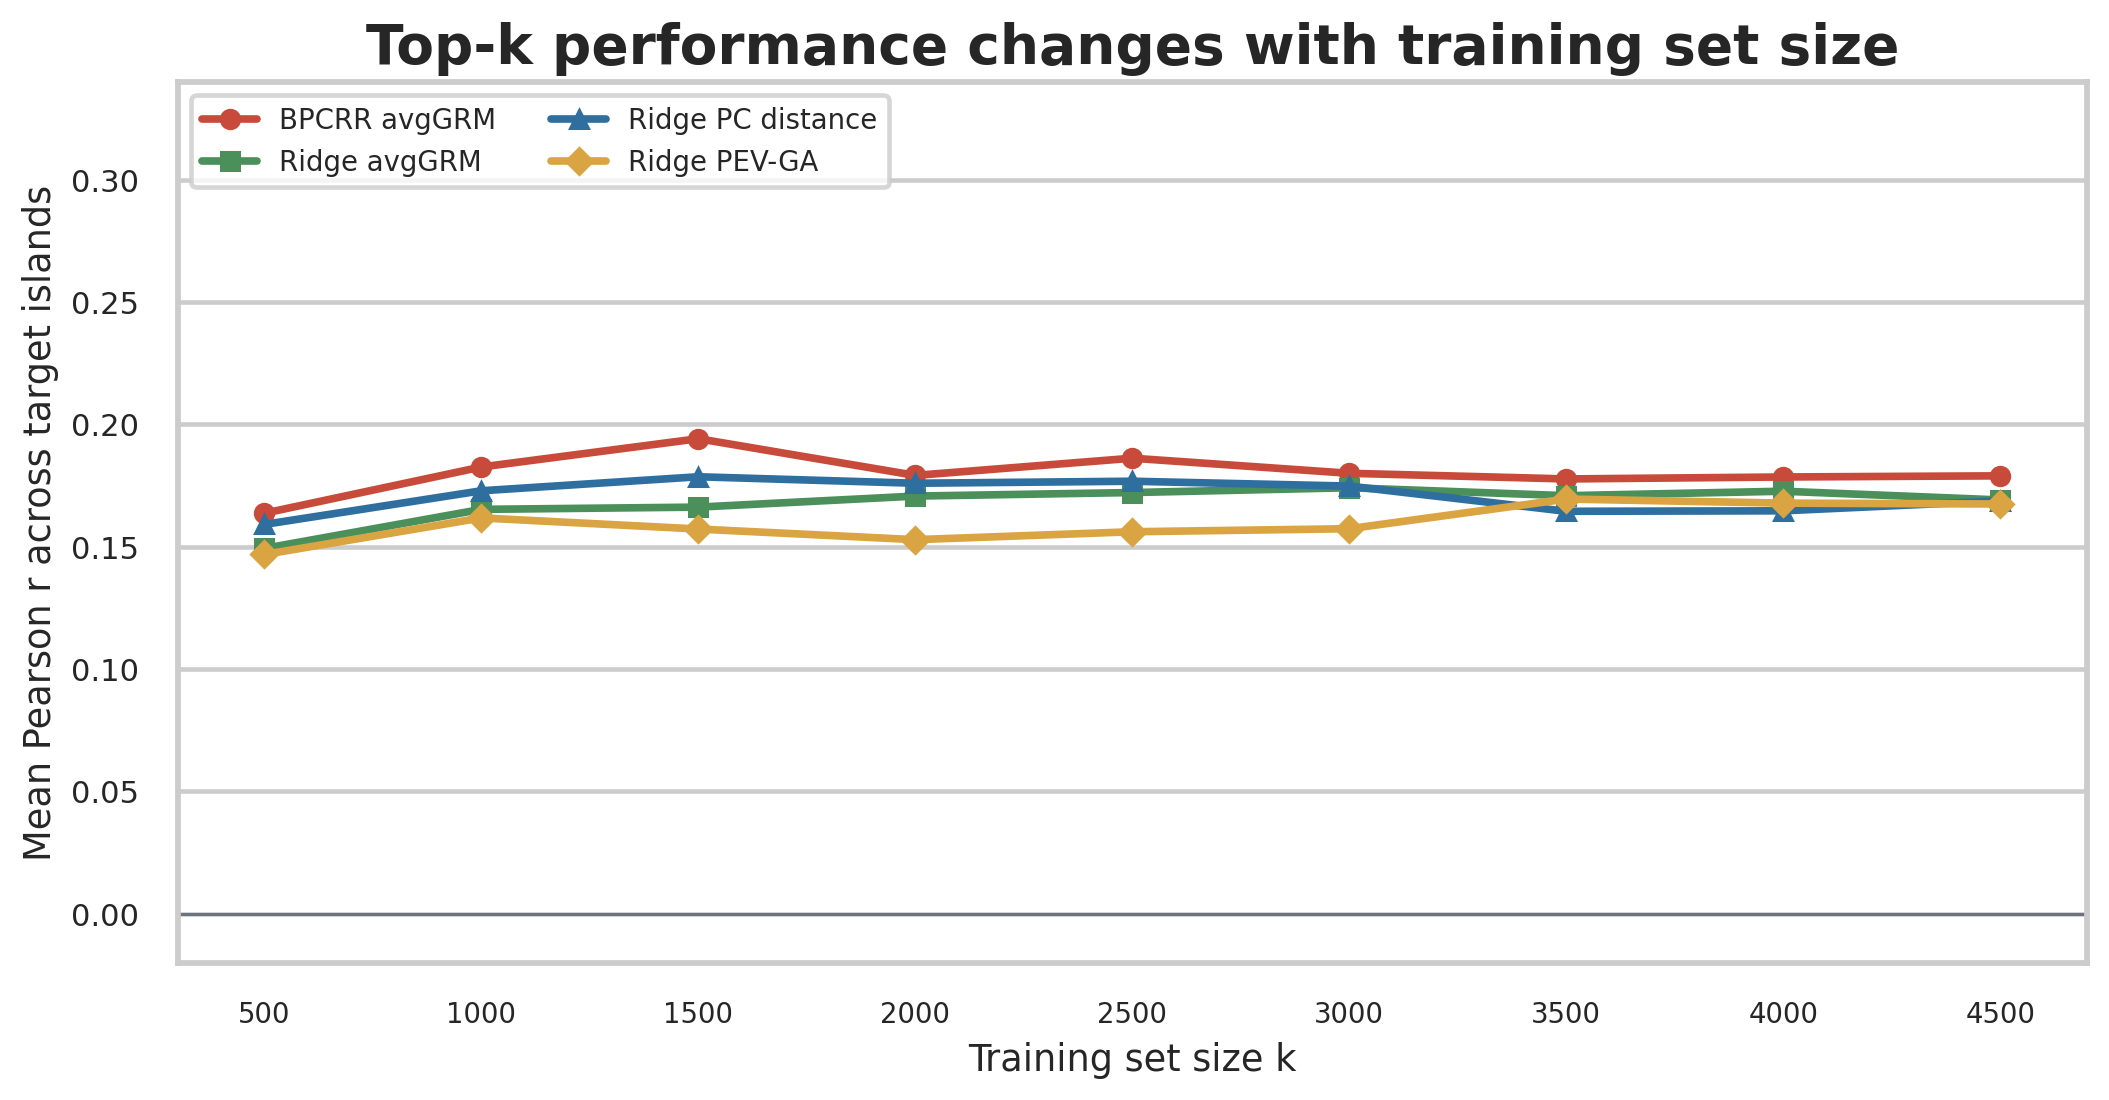
\includegraphics[width=\linewidth,height=0.50\textheight,keepaspectratio]{topk_training_size_lines.png}

  {\small\color{ThesisGray}There may be a useful training-set size, but the best \(k\) is difficult to know a priori and differs by model.}
\end{frame}

\begin{frame}{Nested CV for target-aware rules}
  \begin{columns}[T,onlytextwidth]
    \begin{column}{0.60\textwidth}
      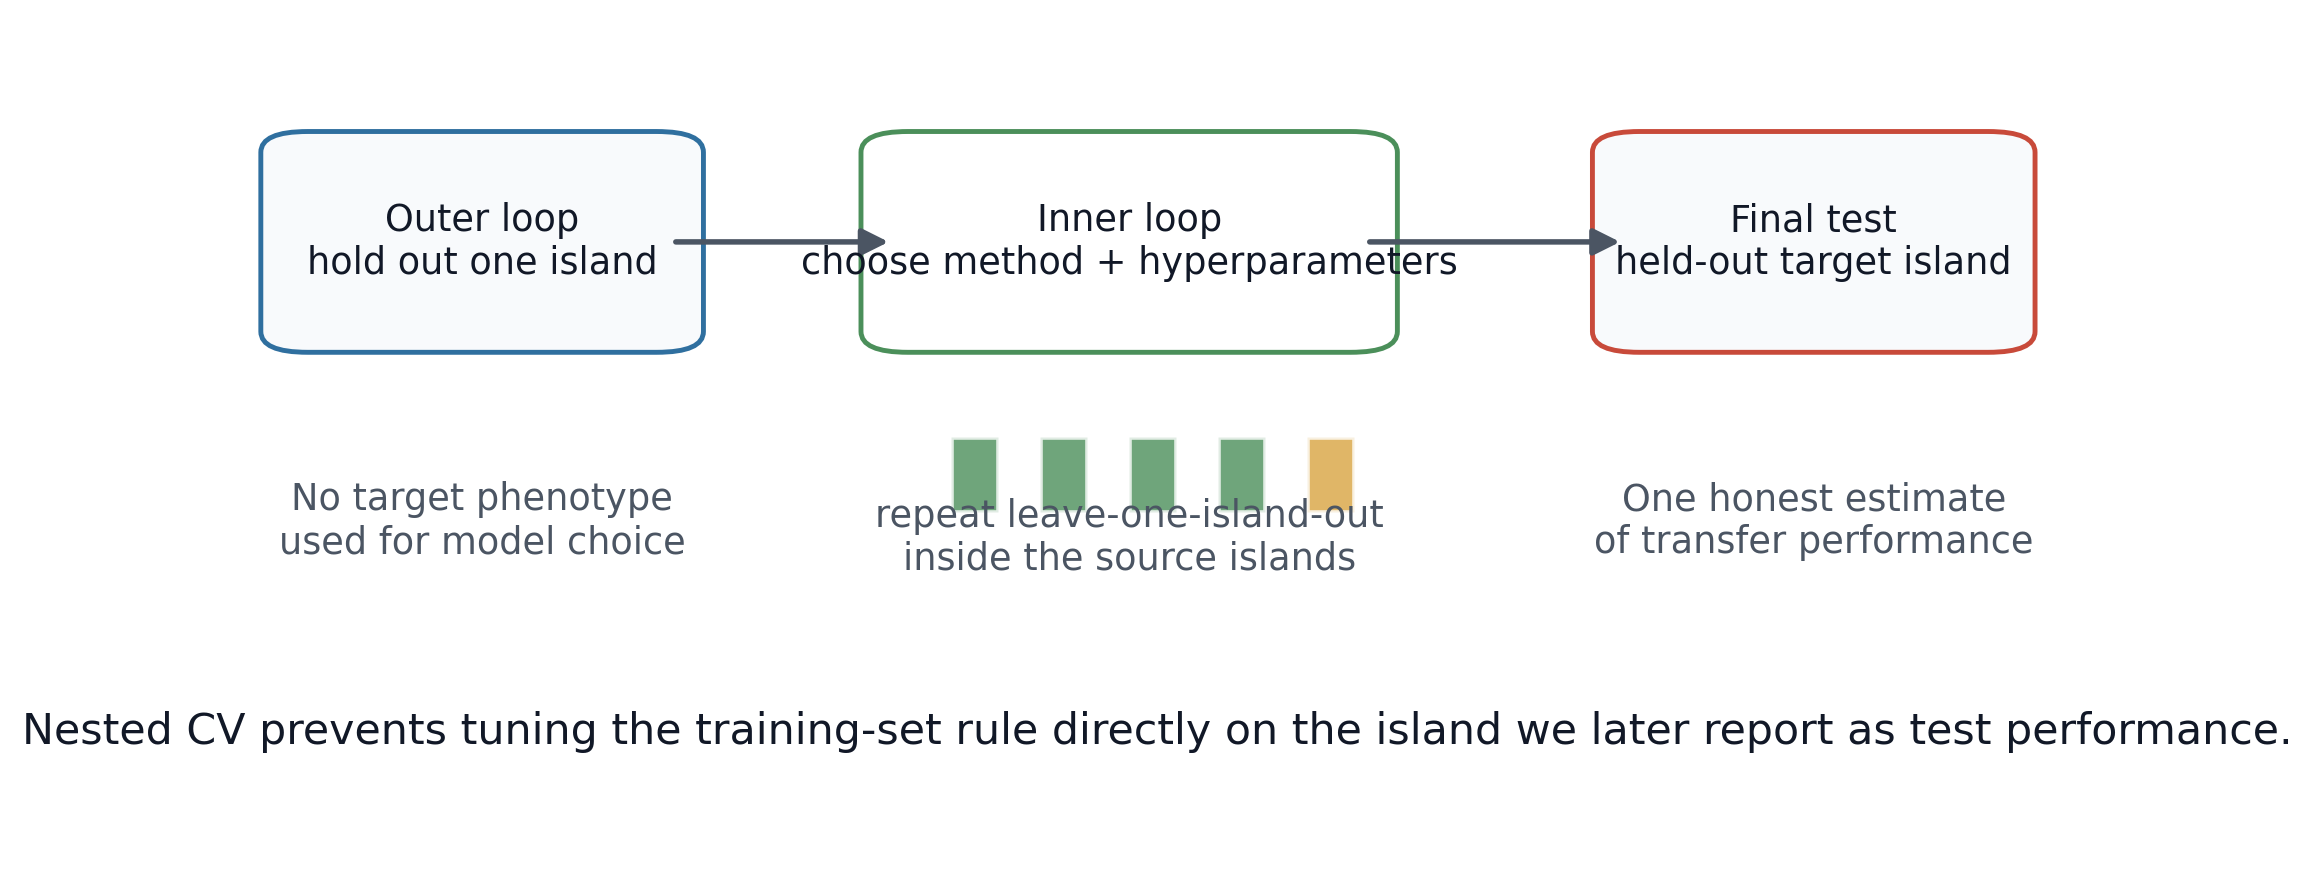
\includegraphics[width=\linewidth]{nested_cv_schematic.png}
    \end{column}
    \begin{column}{0.37\textwidth}
      \small
      \begin{itemize}
        \item Outer loop: hold out the target island.
        \item Inner loop: choose model, weighting rule, and hyperparameters using only source islands.
        \item Final: retrain on all source islands and evaluate once on the target island.
      \end{itemize}
      \takeaway{\small This keeps the reported target performance honest.}
    \end{column}
  \end{columns}
\end{frame}

\begin{frame}{Importance weighting}
  \begin{columns}[T,onlytextwidth]
    \begin{column}{0.48\textwidth}
      \begin{block}{Target risk by source weighting}
      Under covariate shift,
      {\small
      \[
        R_T(f)=\mathbb{E}_{T}\{\ell(f(X),Y)\}
      \]
      \[
        R_T(f)\approx
        \mathbb{E}_{S}\{w(X)\ell(f(X),Y)\}.
      \]
      }
      where
      \[
        w(x)=\frac{p_T(x)}{p_S(x)}.
      \]
      \end{block}
    \end{column}
    \begin{column}{0.48\textwidth}
      \begin{block}{Bayes ratio from a domain classifier}
      Let \(D\in\{T,S\}\) indicate target or source.
      \[
        p(D=T\mid x)=\frac{p(x\mid D=T)p(D=T)}{p(x)}.
      \]
      Therefore
      \[
        \frac{p(x\mid D=T)}{p(x\mid D=S)}
        =
        \frac{p(D=T\mid x)}{p(D=S\mid x)}
        \frac{p(D=S)}{p(D=T)}.
      \]
      \end{block}
    \end{column}
  \end{columns}

  \smallcite{In practice I estimate this with logistic classification in PC space, then clip/smooth weights for stability.}
\end{frame}

\begin{frame}{Importance weighting results}
  \begin{columns}[T,onlytextwidth]
    \begin{column}{0.36\textwidth}
      \small
      \begin{itemize}
        \item Density-ratio weighting was tuned inside nested CV.
        \item The weighted models are close to full-source baselines.
        \item This is more conservative than top-\(k\), but has not clearly improved prediction yet.
      \end{itemize}
      \takeaway{\small Target-aware weighting has not yet given a robust win under strict validation.}
    \end{column}
    \begin{column}{0.62\textwidth}
      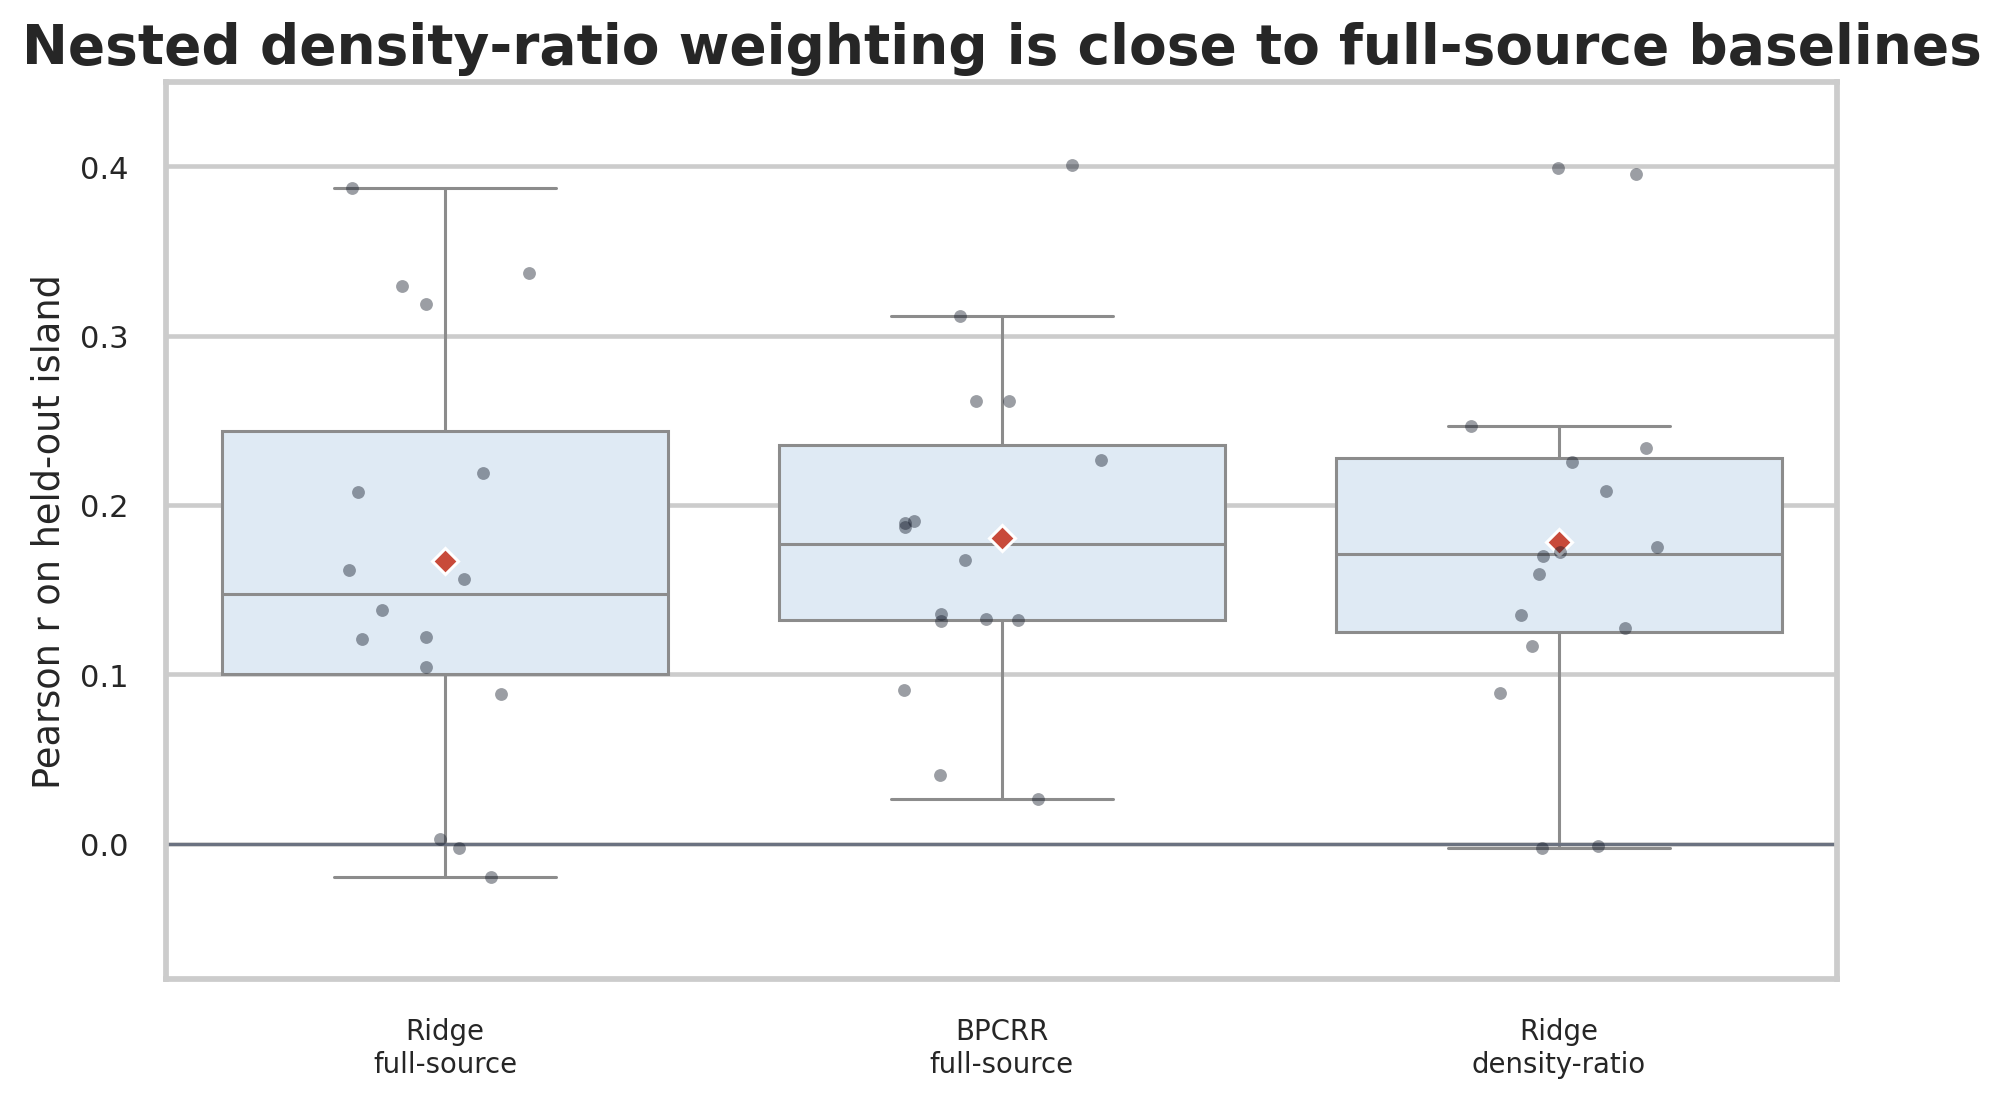
\includegraphics[width=\linewidth,height=0.72\textheight,keepaspectratio]{nested_cv_outer_fold_comparison.png}
    \end{column}
  \end{columns}
\end{frame}

\begin{frame}{Reflections}
  \begin{columns}[T,onlytextwidth]
    \begin{column}{0.48\textwidth}
      \begin{block}{What seems to work}
      \begin{itemize}
        \item Genetic similarity contains signal for training selection.
        \item Top-\(k\) BPCRR/avgGRM gives the clearest preliminary improvement.
        \item Shapley is useful for diagnosing harmful source islands.
      \end{itemize}
      \end{block}
    \end{column}
    \begin{column}{0.48\textwidth}
      \begin{block}{What is hard}
      \begin{itemize}
        \item The best \(k\) is hard to know without target phenotypes.
        \item Shapley is expensive and calibration-dependent.
        \item Weighting can reduce bias, but may increase variance or effective sample-size problems.
      \end{itemize}
      \end{block}
    \end{column}
  \end{columns}

  \vspace{0.4em}
  \takeaway{Future work: better a priori \(k\)-choice, stability diagnostics for weights, and clearer separation of true transfer gain from island-specific noise.}
\end{frame}

\begin{frame}
  \centering
  \Huge Thank you

  \vspace{1em}
  \Large Questions?
\end{frame}

\end{document}
